\begin{solution}

We developed the code based on the skeleton provided in \texttt{parallel.cu}. 
In addition to the basic requirements stated in the 5 steps in the problem statement, we used the constant memory and the shared memory to accelerate the computation. 
In particular, the constant memory is applied to store the constant variables such as \texttt{nx} and \texttt{ny}, and the shared memory is applied to cache the field variable \texttt{\_u} as each of its element would be accessed for multiple times by different threads in one Jacobi iteration. 
Our completed code has been uploaded  \href{https://github.com/iacs-ac290r-2019-2/homework/tree/master/HW2/Group/Problem2}{here}. 
\\
The code is compiled and tested on Odyssey, the HPC cluster maintained by Harvard FAS Research Computing. We observed how the performance scale with the resolution as well as the block dimension. The results are displayed in Figure \ref{fig:p2_res} and Figure \ref{fig:p2_thr}. 

\begin{figure}[H]
    \centering
    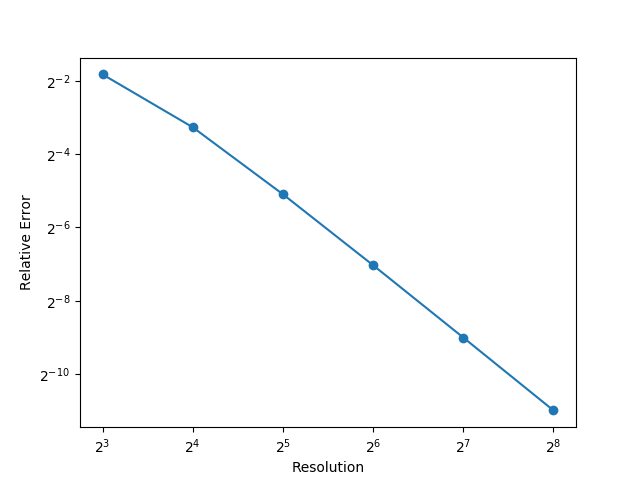
\includegraphics[scale=0.4]{YiqiXie/res_err.png}
    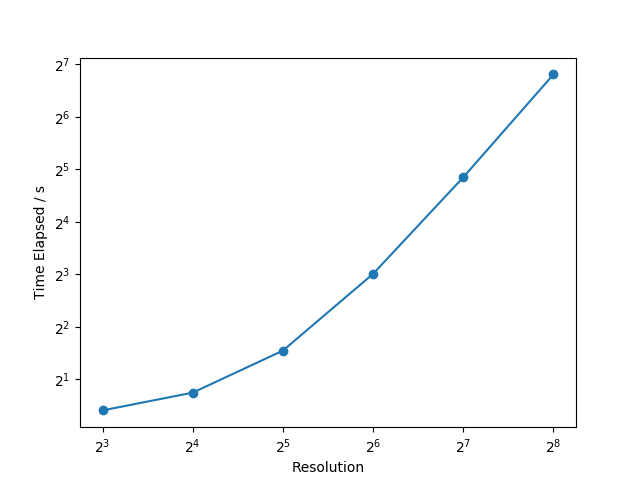
\includegraphics[scale=0.4]{YiqiXie/res_time.png}
    \caption{Performance scale with the resolution. \texttt{MAX\_THREAD\_NUM}=18. }
    \label{fig:p2_res}
\end{figure}

\begin{figure}[H]
    \centering
    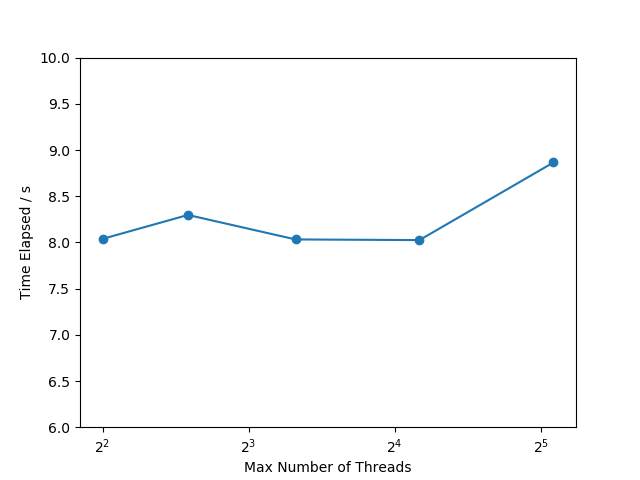
\includegraphics[scale=0.4]{YiqiXie/thr_time.png}
    \caption{Performance scale with the block dimension. The grid is $64\times 64$. }
    \label{fig:p2_thr}
\end{figure}

As we enhance the resolution (denoted by the grid size $N\times N$), we see that the relative error shrinks asymptotically with $O(\frac{1}{N^2})$, and the elapsed time increases asymptotically with $O(N^2)$, which makes sense for our Jacobi iteration setup. On the other hand, the performance does not seem to vary a lot with block dimension. Due to hardware restriction, we cannot try $\texttt{MAX\_THREADS\_DIM}\geq 2^6$. Based on the trend in Figure \ref{fig:p2_thr}, the runtime might increase with larger block dimensions. 

\end{solution}